\documentclass{beamer}

%% Juego de caracteres usado en el archivo fuente: UTF-8
\usepackage{ucs}
\usepackage[utf8x]{inputenc}
\uselanguage{spanish}
%Para la identación del español
\usepackage[spanish]{babel}

% There are many different themes available for Beamer. A comprehensive
% list with examples is given here:
% http://deic.uab.es/~iblanes/beamer_gallery/index_by_theme.html
% You can uncomment the themes below if you would like to use a different
% one:
%\usetheme{AnnArbor}
%\usetheme{Antibes}
%\usetheme{Bergen}
%\usetheme{Berkeley}
%\usetheme{Berlin}
%\usetheme{Boadilla}
%\usetheme{boxes}
%\usetheme{CambridgeUS}
%\usetheme{Copenhagen}
%\usetheme{Darmstadt}
%\usetheme{default}
%\usetheme{Frankfurt}
%\usetheme{Goettingen}
%\usetheme{Hannover}
%\usetheme{Ilmenau}
%\usetheme{JuanLesPins}
%\usetheme{Luebeck}
\usetheme{Madrid}
%\usetheme{Malmoe}
%\usetheme{Marburg}
%\usetheme{Montpellier}
%\usetheme{PaloAlto}
%\usetheme{Pittsburgh}
%\usetheme{Rochester}
%\usetheme{Singapore}
%\usetheme{Szeged}
%\usetheme{Warsaw}

%Para la identación del español
\usepackage[spanish]{babel}

\title{NMAP}

% A subtitle is optional and this may be deleted
%\subtitle{Optional Subtitle}

\author{Jesús Rodríguez Heras \\ Juan Pedro Rodríguez Gracia \\ Javier Holgado Durán \\ Jaime Junquera Melendez \\ Jose Carlos Abollo Palacios}
% - Give the names in the same order as the appear in the paper.
% - Use the \inst{?} command only if the authors have different
%   affiliation.

%\institute[Escuela Superior de Ingeniería] % (optional, but mostly needed)
%{
%  \inst{1}%
%  Department of Computer Science\\
%  University of Somewhere
%  \and
%  \inst{2}%
%  Department of Theoretical Philosophy\\
%  University of Elsewhere}
% - Use the \inst command only if there are several affiliations.
% - Keep it simple, no one is interested in your street address.

%\date{Vulnerabilidades en redes}
% - Either use conference name or its abbreviation.
% - Not really informative to the audience, more for people (including
%   yourself) who are reading the slides online

%\subject{Theoretical Computer Science}
% This is only inserted into the PDF information catalog. Can be left
% out. 

% If you have a file called "university-logo-filename.xxx", where xxx
% is a graphic format that can be processed by latex or pdflatex,
% resp., then you can add a logo as follows:

% pgfdeclareimage[height=0.5cm]{university-logo}{university-logo-filename}
% \logo{\pgfuseimage{university-logo}}

% Delete this, if you do not want the table of contents to pop up at
% the beginning of each subsection:
%\AtBeginSubsection[]
%{
%  \begin{frame}<beamer>{Índice}
%    \tableofcontents[currentsection,currentsubsection]
%  \end{frame}
%}

% Let's get started
\begin{document}

\begin{frame}
  \titlepage
%  \begin{center}
%  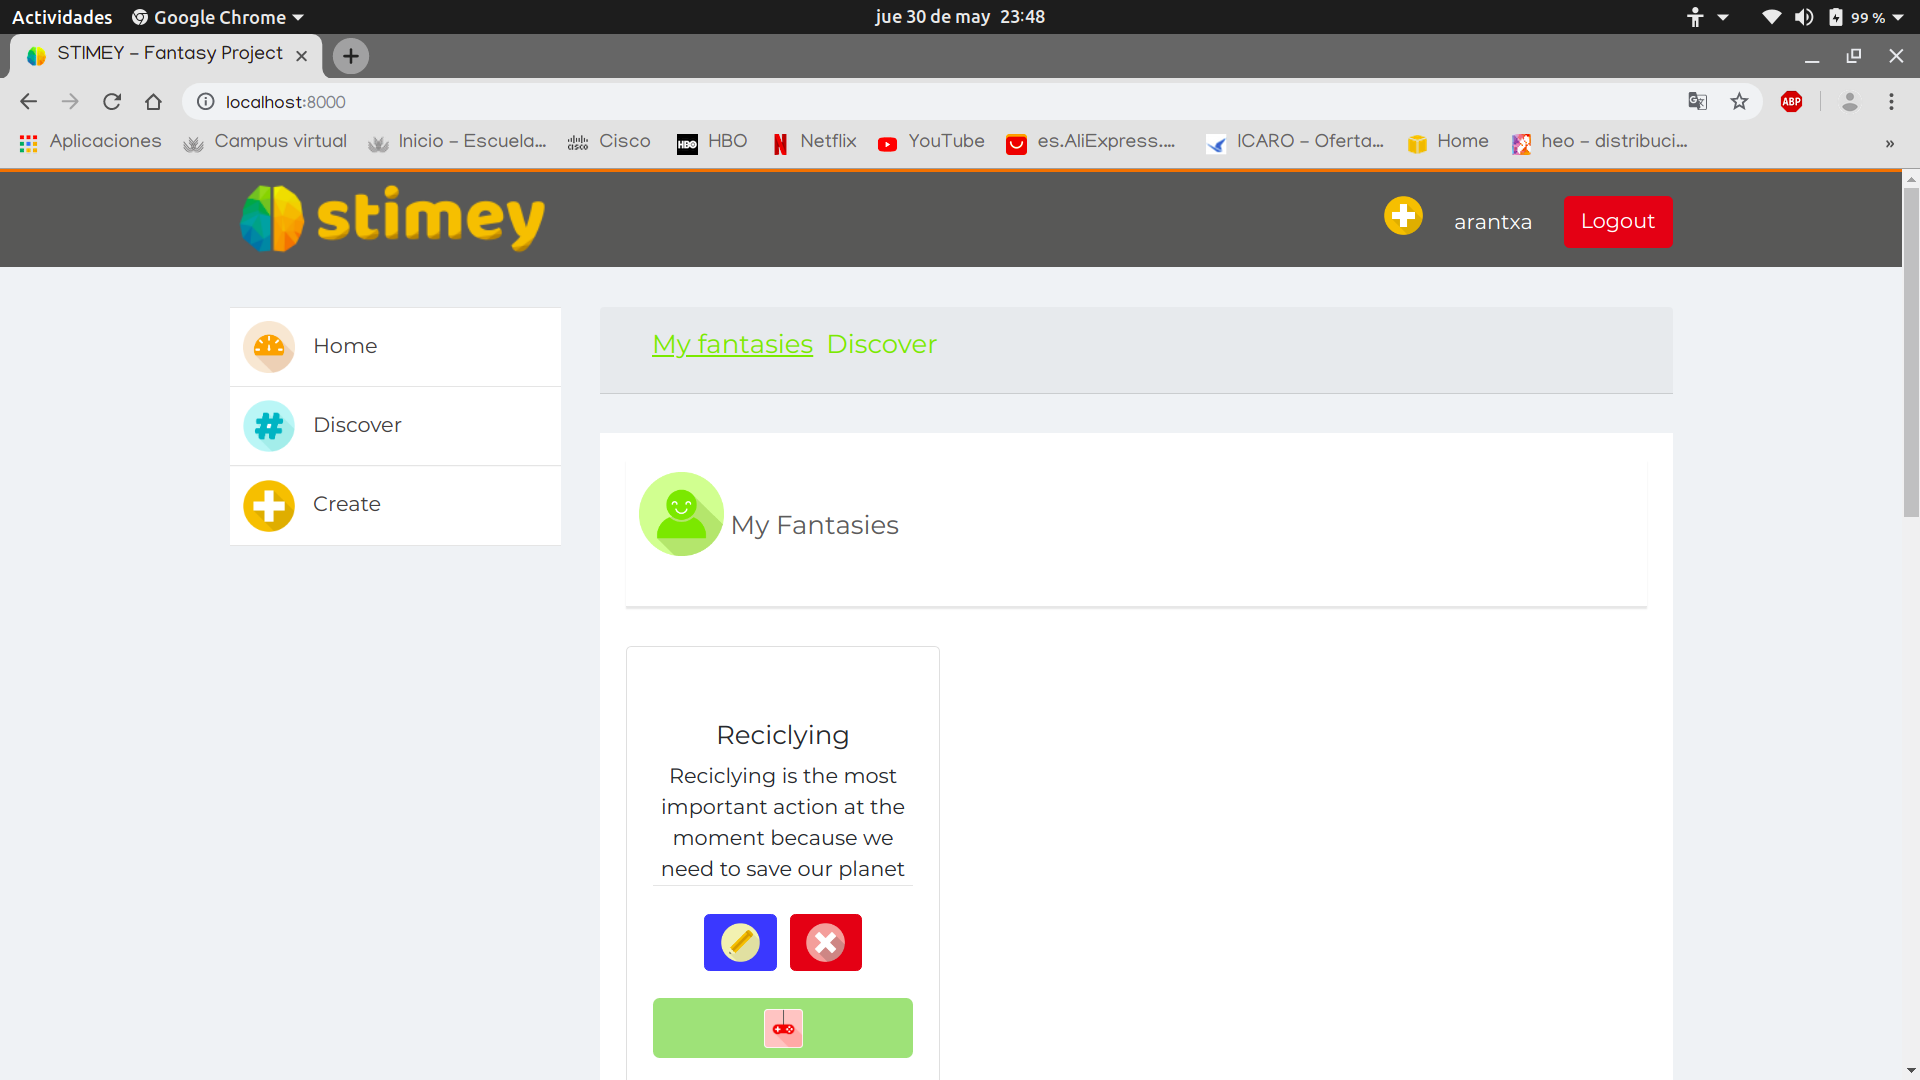
\includegraphics[scale=0.2]{Portada.png}	
%  \end{center}
  
\end{frame}

%\begin{frame}{Índice}
%  \tableofcontents
%  % You might wish to add the option [pausesections]
%\end{frame}

% Section and subsections will appear in the presentation overview
% and table of contents.

\section{Definición}
\begin{frame}{¿Qué es NMAP?}
	\begin{block}{Definición}
		Es un software libre con paradigma de auditoría cuya función es el escaneo de puertos y host de una red. Se puede usar desde consola o desde interfaz gráfica.
	\end{block}
\end{frame}

\section{Características}
\begin{frame}{Características y scripts}
\begin{block}{Características}
	\begin{itemize}
		\item Escaneo de puertos.
		\item Descubrimiento de servidores.
		\item Determinación del sistema operativo de un host.
		\item Mapeo de redes.
		\item Debugeo de interfaces y rutas.
	\end{itemize}
\end{block}
	\begin{block}{Scripts}
		Gracias al uso de scripts puede comrpobar algunas de las siguientes vulnerabiliades.
		\begin{itemize}
			\item \textbf{Malware:} Revisa si hay conexiones abiertas por códigos maliciosos.
			\item \textbf{Vuln:} Descubre las vulnerabilidades más conocidas.
			\item \textbf{Discovery:} Recupera información después de un ataque.
			\item \textbf{All:} Ejecuta todas las anteriores.
		\end{itemize}
	\end{block}
\end{frame}

\section{Ejemplos}
\begin{frame}{Ejemplos}
	\begin{block}{nmap -p 1-65535 -sV -sS -T4 target}
		Obtiene la versión de todos los puertos del objetivo.
	\end{block}
	\begin{block}{nmap -v -sV -O -sS -T5 target}
		Escaneo sigiloso de sistema opeativo y salida verbosa.
	\end{block}
	\begin{block}{nmap --iflist}
		Debugeo de interfaces y rutas.
	\end{block}
\end{frame}

\begin{frame}{Ejemplos}
	\begin{center}
			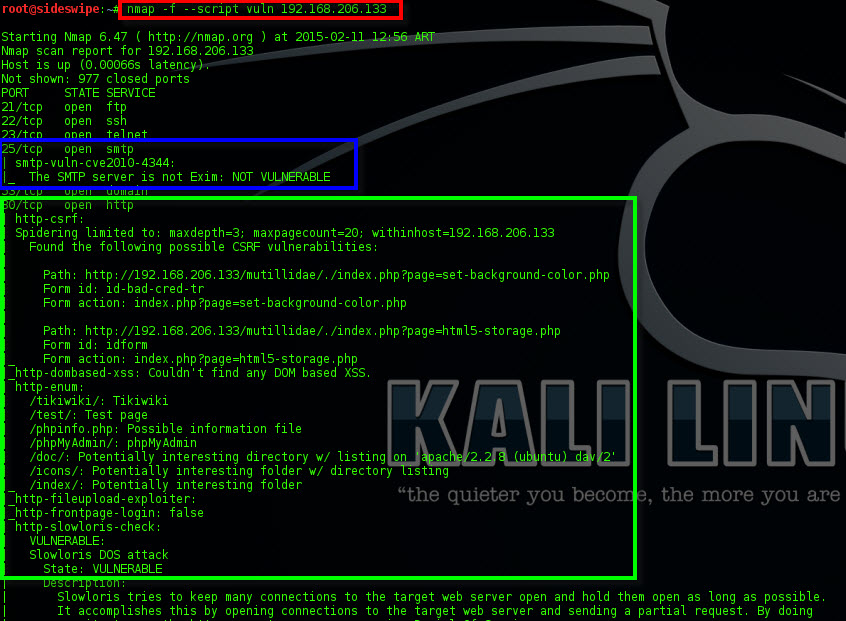
\includegraphics[scale=0.45]{Vuln.jpg}
	\end{center}

\end{frame}

\section{Bibliografía}
\begin{frame}{Bibliografía}
	\url{https://es.wikipedia.org/wiki/Nmap}
	
	\url{https://nmap.org/nsedoc/}
	
	\url{https://www.cyberciti.biz/security/nmap-command-examples-tutorials/}
\end{frame}

\end{document}


